% vim: set textwidth=78 autoindent:

\section{Conventions}\label{label_conventions}
\pagenumbering{arabic}
\setcounter{page}{1}


%%%%%%%%%%%%%%%%8%%%%%%%%%%%%%%%%%%%%%%%%%%%%%%%%%%%
%
% This is a collection of macros to maintain a uniform style throughout
% the user guide.
%
% TEXT STYLES
% These styles change the text appearance but don't add any shadow boxes
% and should be used to refer to non-GUI text (command line, code)
% or non-clickable GUI text (labels).
%
% usertext
% generic style for text that the user should type in from the keyboard
% Note: for user input into a labelled text field in the GUI, see \inputtext
% usage: \usertext{qgis ---help}
\newcommand{\usertext}[1]{\texttt{#1}}

% filename
% usage: \filename{lakes.shp}
\newcommand{\filename}[1]{\texttt{#1}}

% dropmenuopttwo: for dropdown menu items with icons
% usage: \mainmenuopt{Layer} >
% \dropmenuopttwo{mActionAddRasterLayer}{Add a Raster Layer}
\newcommand{\dropmenuopttwo}[2]{%
\raisebox{-6pt}{%
{%
\setlength{\fboxsep}{0pt}%
\shadowbox{\setlength{\fboxsep}{2pt}%
\fcolorbox[rgb]{.95,.95,0.8}[rgb]{.95,.95,0.8}%
{\includegraphics[width=3mm]{#1} \guilabel{#2}}}%
}}}

% button: for any button that only has text, no icon
% usage: \button{Save as Default}
\newcommand{\button}[1]{%
\raisebox{-6pt}{%
\shadowbox{\guilabel{#1}}
}}

% server
% usage: \server{myhost.de}
\newcommand{\server}[1]{\textit{#1}}

% keystroke
% style for user input by individual keystrokes
% usage: \keystroke{p}, \keystroke{Ctrl+B}
\newcommand{\keystroke}[1]{\cornersize{.6}\ovalbox{\textsf{#1}}}

% guilabel
% generic style for text that appears in the GUI
% usage
\newcommand{\guilabel}[1]{\textsf{#1}}

% dialog
% usage: \dialog{Layer Properties}
\newcommand{\dialog}[1]{
\fcolorbox{gray}[rgb]{.95,.95,0.8}{%
\textbf{\textcolor{black}{#1}}}}

% Here are some styles for use only when discussing Python coding
% classname
% usage: \classname{NewLayer}
\newcommand{\classname}[1]{\textsf{\textbf{#1}}}

% object
% usage
\newcommand{\object}[1]{\textsf{\textit{#1}}}

% method
% usage: \method{classFactory}
\newcommand{\method}[1]{\textsf{\textit{#1}}}

% fieldname: part of the set intend to be used to describe Python coding.
% So "field" in this case refers to data members of a class or object, not 
% a "field" from a table or database.
% I have commented out this macro, because it wasn't actually used in the 
% creating_applications section.
% For "fields" from a table or database, use one of the following
% 1. When the field name is something a user should type in, use \usertext
% 2. When the field name is something that the user will see in the GUI, but not 
% click on, use \guilabel
% 3. When the field name is something that the user will select from a selection 
% field, use \selectstring. This requires two parameters, one for the 
% label, the other for the selected text.
%\newcommand{\fieldname}[1]{\textsl{#1}}% 

% ??? these styles are from Gary: use only in 
%\newcommand{\sqltable}[1]{\textsf{\textbf{#1}}}

% CLICKABLE STYLES
% These styles add a shadow box to indicate the user can click on something
% this command sets the shadow size for the entire document
\setlength{\shadowsize}{2pt}%

% Icons for different operation systems
\newcommand{\nix}[1]{\includegraphics[height=5mm]{nix.eps} #1}
\newcommand{\win}[1]{\includegraphics[height=5mm]{win.eps} #1}
\newcommand{\osx}[1]{
\includegraphics[height=5mm]{osx.eps} #1}

% add operation system icons to figure \caption
% usage: \caption{Text \wincaption}
\newcommand{\nixcaption}{\protect\includegraphics[height=4mm]{nix.eps}}
\newcommand{\wincaption}{\protect\includegraphics[height=4mm]{win.eps}}
\newcommand{\osxcaption}{\protect
\includegraphics[height=4mm]{osx.eps}}

% OTHER STYLES
% some styles for the Qt GUI- these are placeholders at present
\newcommand{\qtmainmenuopt}[1]{\textsf{#1}}
\newcommand{\qtdropmenuopt}[1]{\textsf{#1}}
\newcommand{\qtdialog}[1]{\textsf{#1}}


%%%%%%%%%%%%%%%%%%%%%%%%%%%%%% here the section starts %%%%%%%%%%%%%%%%%%%%%

This section describes a collection of uniform styles throughout the manual.
The conventions used in this manual are as follows:

\minisec{Text or Keyboard Conventions}

The manual also includes styles related to text, keyboard commands and coding
to indicate different entities, such as classes, or methods. They don't
correspond to any actual appearance.

\begin{itemize}
%
%Use for all urls. Otherwise, it is not clickable in the document.
\item Hyperlinks: \url{http://qgis.org}
%
\item Single Keystroke: press \keystroke{p}
\item Keystroke Combinations: press \keystroke{Ctrl+B}, meaning press and hold the Ctrl key and then press the B key.
\item Name of a File: \filename{lakes.shp}
%\item Name of a Field: \fieldname{NAMES}
\item Name of a Class: \classname{NewLayer}
\item Method: \method{classFactory}
\item Server: \server{myhost.de}
%\item SQL Table: \sqltable{example needed here}    
%
%Use usertext for all other text that the user must enter from the keyboard
%that is not covered by any of the above cases
\item User Text: \usertext{qgis ---help}
\end{itemize}

Code is indicated by a fixed-width font:
\begin{verbatim}
PROJCS["NAD_1927_Albers",
  GEOGCS["GCS_North_American_1927",
\end{verbatim}

\minisec{Platform-specific instructions}

This indicates that on Linux, Unix and Windows platforms you need to follow
different instructions. Larger amounts of text may be formatted as a list:

\begin{itemize}
\item \nix{do this;} 
\item \win{do that;} 
\item \osx{do something else.}
\end{itemize}

or as paragraphs.

\nix{} \osx{} Do this and this and this. Then do this and this and this
and this and this and this and this and this and this.

\win{}Do that. Then do that and that and that and that and that and that and
that and that and that and that and that and that and that and that and that.

Screenshots that appear throughout the user guide have been created on
different platforms; the platform is indicated by the platform-specific icons
at the end of the figure caption.



